\documentclass{pset}
\usepackage{jdh}
\usepackage{indentfirst}
\usepackage[T1]{fontenc}
\usepackage{graphicx}

\renewcommand\maketitle{
  \vspace*{-5em}
  \begin{center}\framebox{\parbox{\boxlength}{\bf
    CS 4780, Fall 2013\hfill Final Report\hfill 11 December 2013
  }}
  \end{center}
  \vspace{1em}
}


\begin{document}

\maketitle

\section{Introduction}
Salary transparency is a woefully underdeveloped concept in the United States.
Historically, it has been in an employers best interests to keep job salaries
as private as possible, allowing them to negotiate on an individual level and
suppress competition on compensation. Websites such as Glassdoor have attempted
to address this problem through anonymous salary postings by current employees,
but these postings can vary widely and offer no guarantee of a decent wage for
potential employees. The true solution to this problem is a public listing of
starting salary for a position; a concept that has been embraced by many
employers in the United Kingdom. Unfortunately, not all firms have adopted this
attitude, and about half of all current job postings do not provide salary
information to applicants. Our algorithm aims to fix this by providing an
accurate estimate of a position's salary from the information in the listing
alone. 

We approach this problem by applying a variety of different machine learning
techniques, including generative and discriminative models, which we will then
combine to get a final prediction. Initially, we had planned to combine the
algorithms via boosting, however we later discovered a more effective strategy
was to structure them hierarchically based on their relative strengths. This
produced strong results, correctly classifying over 90\% of the positions in
our test set within 2,500\textsterling of their actual yearly salary. Average
error across our 50,000 record test set was about 27444\textsterling, about
7.8\% of the average job salary.  

\section{Problem Definition and Methods}

\subsection{Task Definition}
Our task is to accurately predict the yearly salary of a job listing from the
UK given only the information in its listing. This data includes the job title,
text description, normalized location, contract type and time, sector or
category, and employer. To do this, we were given a training set containing
normalized salaries as well as this information for 244,768 positions.

This problem is interesting for a number of reasons, not in the least because
of its real world implications. From a technical perspective, this is a very
interesting problem because it correlates the relatively small text
descriptions for each position to a large, continuous range. This, combined
with the large data set, gives us a variety of possible strategies. Beyond our
large data set, we also identified over half a million unique features, with
far more possible, allowing fine grained analysis of the data.

\subsection{Algorithms and Methods}
We used a number of different classifiers to arrive at our final prediction.
Since the many of the classifiers we learned were geared toward discrete
classes instead of continuous values, we began by bucketing the data into a
series of classes, each 5000\textsterling wide. This produced the distribution
of label values seen in the figure below.\\
\centerline{\includegraphics[scale=0.5]{fullDist}}\\

We next processed the data, presented as a CSV, into SVM-light format. To
perform the feature identification required for the SVM-light format, we used a
different technique depending on the field of the data. For the text
description, we treated the content like a bag of words, as in the astrophysics
problem from homework 4. Unfortunately, because of the size of the data, we
were unable to evaluate anything besides 1-grams. For other fields, such as
employer, location, and category, we treat as specific features.  A notable
exception to this is the job title category, which in which each word in the
title is considered a unique feature. The reasoning behind this was that terms
such as ``Java Developer'' and ``Java Programmer'' are likely correlated, while
terms such as ``Johnson \& Johsnon'' and ``S.C. Johnson'' may not. This analysis
yielded 521,376 unique features on the provided data.

We next trained three separate classifiers - a Naive Bayes, an optimized SVM,
and ID3 - with the intent of boosting the final products together. After a grid
search for the best parameters, we saw solid results from our SVM, selecting
the correct bucket for about 85\% of our samples. Unfortunately, Bayes and ID3
were far out shown by the optimized SVM, while still taking prohibitively long
to train. 
 
We unsuccessfully attempted to reconcile the poor performance through boosting.
This was done through a modified ADABOOST algorithm for multi-class assignment
given a set of classifiers and their predictions, based upon
http://www.stanford.edu/~hastie/Papers/samme.pdf. However, the difference in
the strength of the classifiers combined with the overlap of which training
instances were incorrectly classified by each approach appeared to cause the
boosting to be unsuccessful. Despite thousands of iterations, we were unable to
force the boosted to algorithm to ever choose against the SVM. 

Scrapping the boosting, we focused on correctly classifying the high income,
low frequency samples that were often missed by the SVM. To do this, we decided
to do a binary split on the data based on a position's salary. We set a cutoff
threshold $\theta$ such that all jobs falling in bucket $\theta$ or below were
put in $G_1$, while those strictly greater than $\theta$ were placed in $G_2$.
$\theta$ was selected such that $|G_1| \approx |G_2|$, which yielded $\theta =
6$. We built an binary SVM classifier for this, as well as two separate
multi-class SVM's for the values in $G_1$ and $G_2$. By allowing the binary SVM
to determine a likely group for a test sample and then feeding that sample into
the appropriate SVM, we were able to substantially increase of accuracy past
the single SVM case. 

Finally, to assign an actual numeric salary to each test case, we trained a
separate ID3 classifier for each label. These were built off a small subset of
samples for that bucket and were given specific salaries as labels, instead of
bucketed values. After the multi-stage SVM classified a sample, it is passed to
the appropriate ID3 classifier, which outputs our final predicted salary.

\section{Experimental Evaluation}

\subsection{Methodology}
Though the Kaggle competition did give us a test set, this set did not provide
us any way to assess our accuracy. Instead, we split our provided training set
into a training set of one-hundred thousand records, test set of fifty-thousand
records, and a validation set of ninety-thousand records. We realize this is a
bit of an odd training-validation split, however our computing resources often
limited us to evaluating only a subset of each, so the total size was fairly
irrelevant. Each set consisted of a random set of samples, so it constituted a
realistic sampling from the distribution. 

Initially, we used the methods listed in section 2.2, forgoing the ID3 step, to
produce a bucket prediction, and then evaluated accuracy using a 0-1 loss
function. To evaluate final accuracy, we included the ID3 step to produce an
actual salary prediction. We compared this prediction to the actual value and
used the absolute value of the difference as our error.

We performed grid search on each SVM using an appropriate subset of the
validation set (IE only high examples for the $G_2$ SVM). The graphs for this
search for the binary classifier and the $G_1$ SVM can be seen below.\\
\centerline{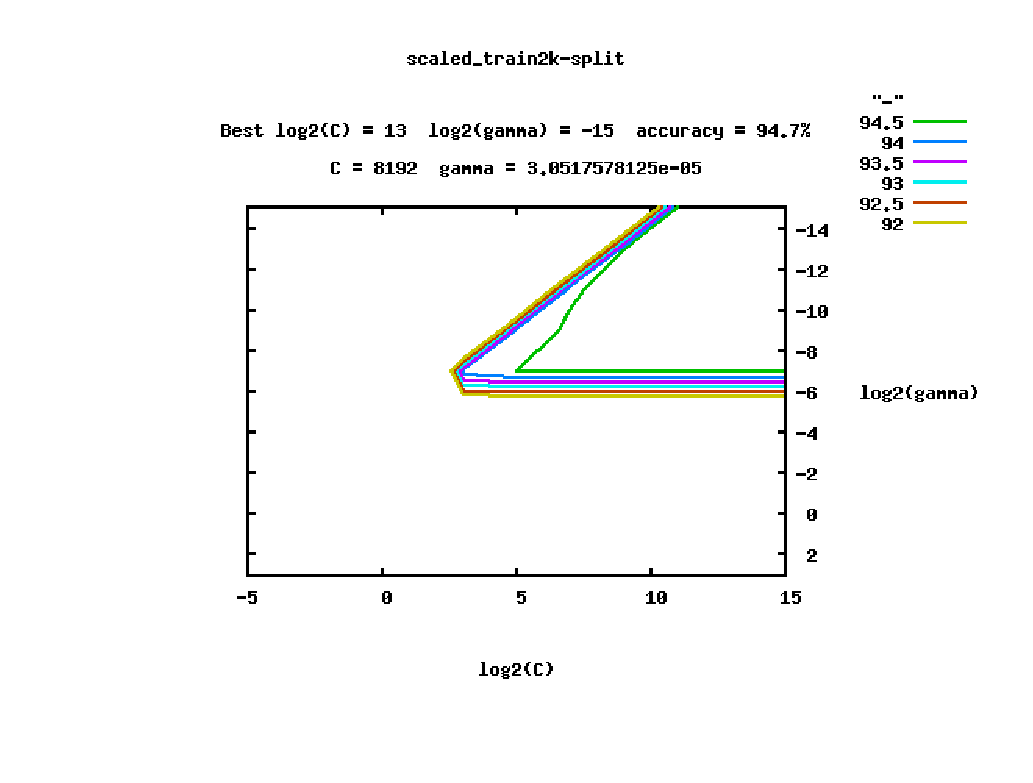
\includegraphics[scale=0.6]{binaryGridSearch}}\\
\centerline{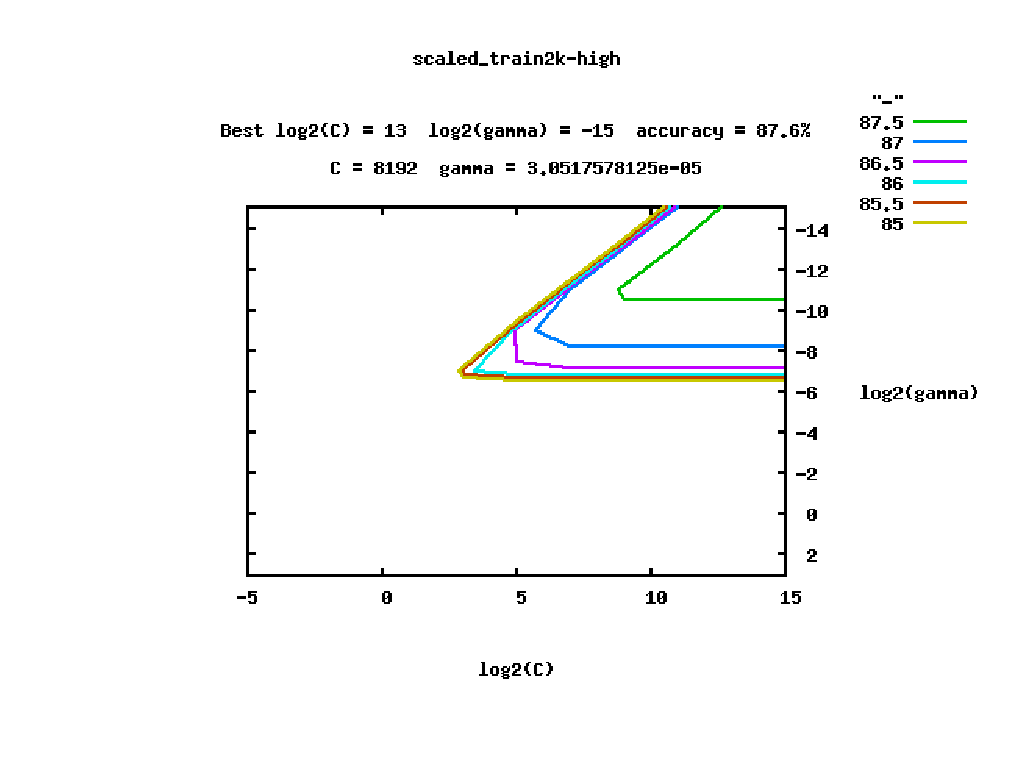
\includegraphics[scale=0.6]{highGridSearch}}\\ We evaluated these
accuracies on fifty-thousand records from the test set, due to computational
limitations. To evaluate baseline bucket accuracy, we produced a set of
fifty-thousand ``predictions'' from a random Poisson process. To most closely
match our data, we used a $\lambda$ of 6 for this process. We also evaluated
relative performance between the different classifiers using a McNemar test.
This was primarily for determining whether or not our multi-stage SVM was
actually an improvement.

\subsection{Results} Our final bucket prediction algorithm had an accuracy of
92.58\%. The final salary prediction gave an average difference of
1569.02\textsterling and an average percent difference of 6.10\%. This is far
better than our baseline Poisson distribution, which had an accuracy of
10.09\%. Below, you can see graphs for our precision and recall percentages by
bucket.\\
\centerline{\includegraphics[scale=0.5]{precisionDistribution}}\\
\centerline{\includegraphics[scale=0.5]{recallDistribution}}\\
Our ID3 and Bayes classifiers did not fair as well, with respective accuracies of 60.37\% and 48.51\%. Note: this Bayes' accuracy is lower than we had initially thought due to mistakenly testing on the wrong set. 

\subsection{Discussion} We felt that, given the range of salaries and
unstructured nature of the problem, our results were very strong. Even our
basic optimized SVM far outperformed the other classifiers, though the
optimization process was intensive. This seems to indicate a level of
complexity within the problem, which could be the root of the simpler
classifier's poor performance. 

We found the strong performance of the multi-level SVM very interesting.
Intuitively, we expected this SVM to perform similarly to our basic one; in
fact, we initially implemented only to force the SVM to predict the higher
labels more frequently, as these would have hurt our accuracy more when moving
from a 0-1 loss function. However, the high level of accuracy when selecting
$G_1$ or $G_2$ seems to indicate there are strong statistical differences
between the two sets. Additionally, the increase in accuracy within each set
seems to indicate that many features' value was context specific, IE a set of
terms could reliably indicate one label when restricted to a subset of the
entire domain. 

Finally, the ID3 forest used for final salary assignment indicates that fine
grain prediction was possible and tractable once we had sufficiently narrowed
down the field. The predictions from these trees performed significantly better
than simple outputting the mean of the bucket. The trees also allow us to see
what features have the most bearing on salary on a more granular scale. 

We realize our methods do present some weaknesses. Mainly, an averaged KNN
implementation would likely fair better than the ID3 setup we have.
Additionally, we are capitalizing on the Poisson nature of the distribution we
have; jobs lacking salary information may not follow this distribution.  

\section{Related Work}

A main source of information of related work on this exact problem can be found
on the Kaggle website forums. It seems that a lot of people decided not to
leave data as raw as we did, doing a lot of processing to the words such as
term frequency-inverse document frequency and other measures. The benefit of
this would be to extract extra information from the words.
However, our group decided that the actual text of
each description was probably less useful than other information we were given.
A lot of groups seemed to overlook the importance of location, and our
representation uses that to a pretty large degree. 

Some of the top Kaggle competitors had lots of success using neural networks
and taking features of n-grams in addition to the other information given.
Being able to implement a neural net in addition to our classifiers would have
been very useful and interesting as these are obviously not easily separated
with a linear classifier. We cannot directly compare our answers using test
sets from the Kaggle competition, so it is tough to compare our mean average
error with the other competitors. After running our algorithm we get an average
error of about 2500, and Kaggle users seem to think that under 4000 or 3000 is
a good result. Our average could be artificially low depending on the actual
test sets, but it seems that our approach is relatively successful.

\section{Future Work}

A main shortcoming of our method is that we did not use feature pruning or any
sort of selection. With our method we were able to get high accuracies with
just our initial idea of what features would be useful. It is probable that
some of the features are noisier and confuse our machine learning models or
that some features are incredibly important but not weighted highly. Using
feature selection methods such as LASSO could potentially provide another boost
in prediction accuracy.

Though we chose not to do regression on our set of salary predictions because
we hypothesized our solution would be more accurate, it would be interesting to
analyze the data using regression-based models. This could be implemented
through support vector machines, our strongest models, as a baseline to compare
against our current prediction model. Maybe even a combination of our binary
classifier and one or several regression based models working in tandem with
binary split could be tested. If it turns out that regression is not as
accurate, the method we used has potential as an alternative. 

Because of the success of the SVM approach, it would be interesting to see if
we could modify the SVM to optimize on the Kaggle defined error rather than 0/1
loss as it does. We optimize the placement into each bucket assuming that any
error is equal, but it is clear that placing a 100,000 salary job into the
5,000 bucket is significantly more damaging to our final error than putting a
100,000 salary into the 95,000 bucket. It seems like an optimization problem
possibly outside the scope of this class, but it certainly could find better
classifications to buckets. 

If we had realized the strength of multi-level hypotheses earlier, we would
have liked to try out different setups. For instance, how many levels are
optimal? What is the best classifier for each level? As we saw, while the ID3
performed poorly overall, it excelled on the fine grain salary prediction; it
would be very interesting to see situations in which Bayes or KNN outperforms
the other classifiers.

Applications of salary prediction would also probably have other information,
which could be a point of future work. For example, if an individual is looking
for a job, their demographic information and past work experience could play
a significant role in salary. We could fill in some features from job advertisements, and ask
individuals for additional information. More features which are relevant should
raise accuracy. 

\section{Conclusion}
On a social level, these results are important as they indicate you can
accurately predict the salary of a job given only it's listing. As outlined in
our intro, this could lead to a much needed increase in the transparency of
starting salaries in the job market. On a technical level, these results are
interesting because they show the strength of a multi-tiered hypothesis versus
a singular classifier. While this may not always be an optimal strategy, this
project should inspire others working on similar problems to experiment with
multi-stage setups. Furthermore, our higher and lower level classifiers are
modular enough to be combined with other mid-level classifiers; if someone else
has reached a higher level bucket accuracy, they should be able to boost their
final results by including one of our stages.

\end{document}
